\section{Experiments \& Results}

The experiments were run in two Parts; Part 1- A classification task to classify a dataset containing 3 classes and 
Part 2- A classification task to classify the `MNIST' dataset.

\subsection{Part 1}

The aim of this part was to verify that the program 
worked. The dataset used in this section is shown in Fig \ref{fig: Synthetic data}.
The dataset was generated such that it would be linearly 
separable. This would facilitate the verification process
since generating a discriminant function for a linearly 
separable dataset is a trivial task for a Neural Network
using non-linear activation functions. 

This simple classification task was also used as a means
to study the activation functions; \textbf{Rectilinear Unit}, 
\textbf{Sigmoid} and \textbf{Hyperbolic tan}. Thus, several
architectures were employed, each being composed of 
one of the 3 activation functions for all its hidden layers.


\begin{figure}
    \centering
    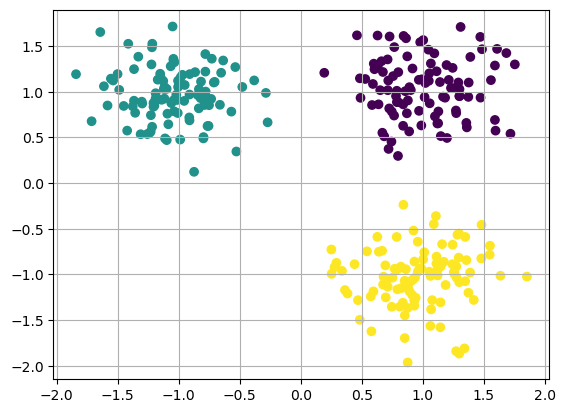
\includegraphics[width=0.5\textwidth]{part_1_data.png}
    \caption[short]{Synthetic data}
    \label{fig: Synthetic data}
\end{figure}
